\chapter{Gated Recurrent Units (GRUs) (2014)}

\begin{figure}[H]
    \centering
    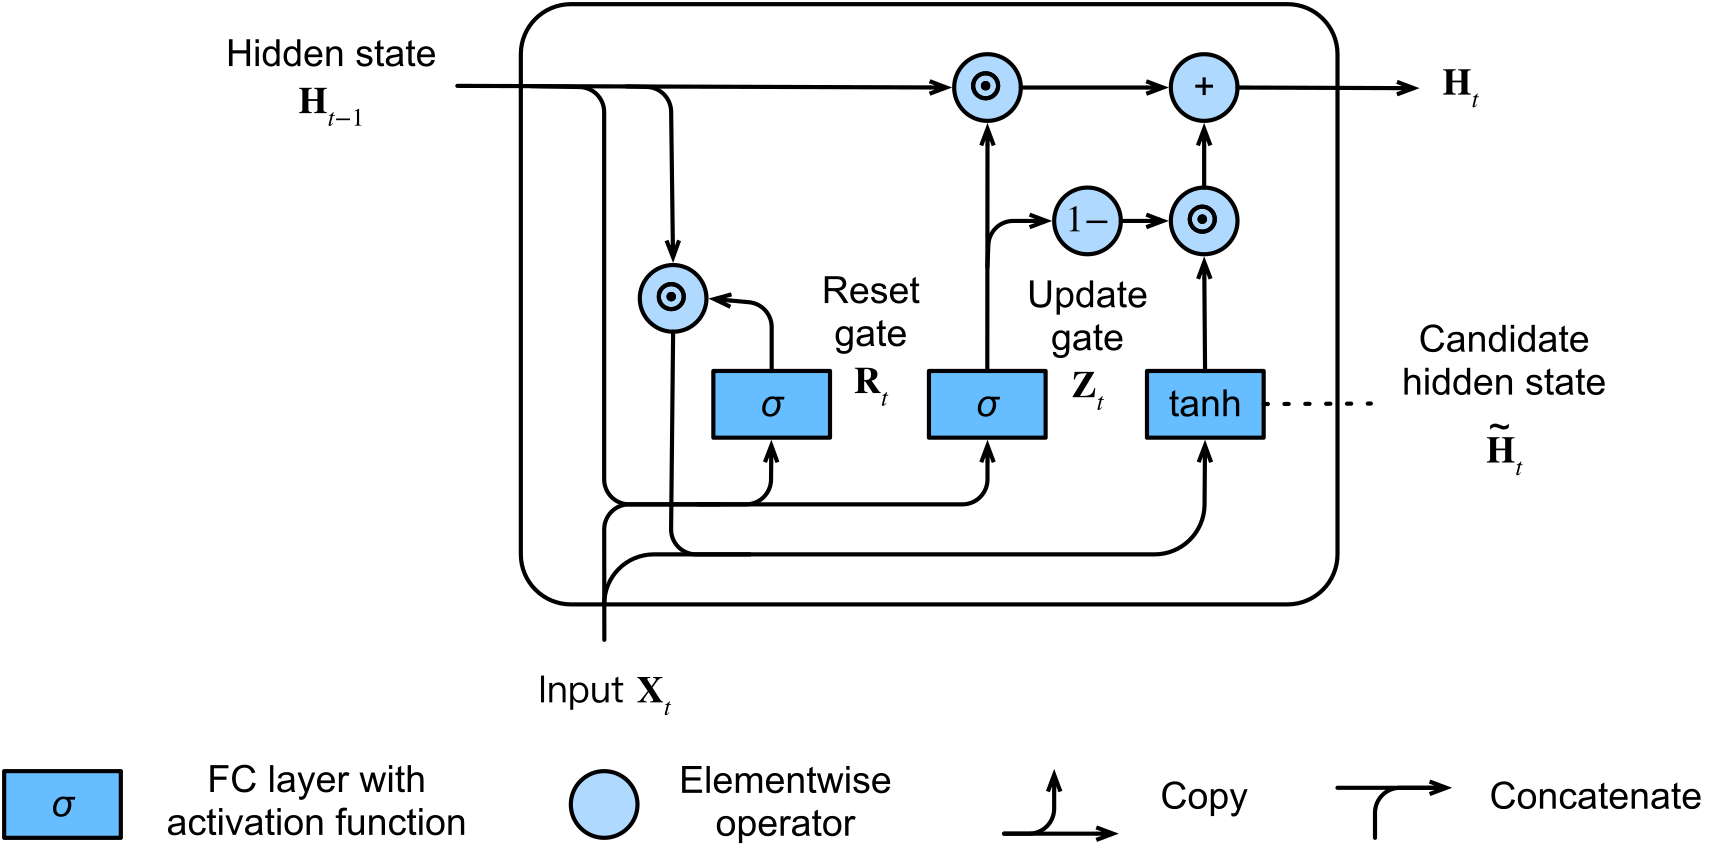
\includegraphics[
        width=\linewidth,
        height=6cm,
        keepaspectratio,
    ]{images/recurrent-neural-networks/gru-arch.png}
    \caption{GRU Architecture}
\end{figure}



\begin{enumerate}
    \item Gated Recurrent Unit (GRU) was introduced which uses LSTM architecture by merging its gating mechanisms offering a more efficient solution for many sequential tasks without sacrificing performance.
    \hfill \cite{geeksforgeeks/machine-learning/gated-recurrent-unit-networks}

    \item The core idea behind GRUs is to use gating mechanisms to selectively update the hidden state at each time step allowing them to remember important information while discarding irrelevant details.
    \hfill \cite{geeksforgeeks/machine-learning/gated-recurrent-unit-networks}

    \item The GRU consists of two main gates:
    \begin{enumerate}
        \item \textbf{Update Gate} ($z_t$): This gate decides how much information from previous hidden state should be retained for the next time step.
        \hfill \cite{geeksforgeeks/machine-learning/gated-recurrent-unit-networks}

        \item \textbf{Reset Gate} ($r_t$): This gate determines how much of the past hidden state should be forgotten.
        \hfill \cite{geeksforgeeks/machine-learning/gated-recurrent-unit-networks}
    \end{enumerate}

    % \item 
\end{enumerate}



\section{Working of GRU}

\begin{enumerate}
    \item \textbf{Reset gate}: $r_t=\sigma(W_r \cdot [h_{t-1},x_t])$
    \hfill \cite{geeksforgeeks/machine-learning/gated-recurrent-unit-networks}
    \\[0.2cm]
    The reset gate determines how much of the previous hidden state $h_{t-1}$ should be forgotten.
    \hfill \cite{geeksforgeeks/machine-learning/gated-recurrent-unit-networks}

    \item \textbf{Update gate}: $ z_t=\sigma(W_z \cdot [h_{t-1},x_t]) $
    \hfill \cite{geeksforgeeks/machine-learning/gated-recurrent-unit-networks}
    \\[0.2cm]
    The update gate controls how much of the new information $x_t$ should be used to update the hidden state.
    \hfill \cite{geeksforgeeks/machine-learning/gated-recurrent-unit-networks}

    \item \textbf{Candidate hidden state}: $ h_t^\prime=\tanh(W_h \cdot [r_t \cdot h_{t-1},x_t]) $
    \hfill \cite{geeksforgeeks/machine-learning/gated-recurrent-unit-networks}
    \\[0.2cm]
    This is the potential new hidden state calculated based on the current input and the previous hidden state.
    \hfill \cite{geeksforgeeks/machine-learning/gated-recurrent-unit-networks}

    \item \textbf{Hidden state}: $ h_t=(1-z_t) \cdot h_{t-1}+z_t \cdot h_t^\prime $
    \hfill \cite{geeksforgeeks/machine-learning/gated-recurrent-unit-networks}
    \\[0.2cm]
    The final hidden state is a weighted average of the previous hidden state $h_{t-1}$ and the candidate hidden state $h_t^\prime$ based on the update gate $z_t$.
    \hfill \cite{geeksforgeeks/machine-learning/gated-recurrent-unit-networks}
\end{enumerate}


\begin{lstlisting}[
    language=Python,
    caption=GRU from scratch (PyTorch) \cite{common/online/chatgpt}
]
class ManualGRU(nn.Module):
    def __init__(self, input_size, hidden_size, output_size):
        """
        Single-layer GRU implemented without using nn.GRU / nn.GRUCell.
        Uses separate parameter chunks for gates:
          z_t = sigmoid(x W_z + h U_z + b_z)
          r_t = sigmoid(x W_r + h U_r + b_r)
          n_t = tanh( x W_n + (r * h) U_n + b_n )
          h_t = (1 - z_t) * n_t + z_t * h
        """
        super().__init__()
        self.input_size = input_size
        self.hidden_size = hidden_size
        H = hidden_size

        # Input -> gates (z, r, n) : shapes (input_size, H)
        self.Wx_z = nn.Parameter(torch.randn(input_size, H) * 0.1)
        self.Wx_r = nn.Parameter(torch.randn(input_size, H) * 0.1)
        self.Wx_n = nn.Parameter(torch.randn(input_size, H) * 0.1)

        # Hidden -> gates (z, r, n) : shapes (H, H)
        self.Wh_z = nn.Parameter(torch.randn(H, H) * 0.1)
        self.Wh_r = nn.Parameter(torch.randn(H, H) * 0.1)
        self.Wh_n = nn.Parameter(torch.randn(H, H) * 0.1)

        # biases for each gate
        self.b_z = nn.Parameter(torch.zeros(H))
        self.b_r = nn.Parameter(torch.zeros(H))
        self.b_n = nn.Parameter(torch.zeros(H))

        # final classifier from last hidden state
        self.Why = nn.Parameter(torch.randn(H, output_size) * 0.1)
        self.by = nn.Parameter(torch.zeros(output_size))

    def forward(self, x, h0=None):
        """
        x: (batch, seq_len, input_size)
        returns logits (batch, output_size) and last hidden (batch, hidden_size)
        """
        batch, seq_len, _ = x.shape
        H = self.hidden_size

        if h0 is None:
            h = x.new_zeros(batch, H)
        else:
            h = h0

        for t in range(seq_len):
            xt = x[:, t, :]  # (batch, input_size)

            # update gate z
            pre_z = xt @ self.Wx_z + h @ self.Wh_z + self.b_z
            z = torch.sigmoid(pre_z)

            # reset gate r
            pre_r = xt @ self.Wx_r + h @ self.Wh_r + self.b_r
            r = torch.sigmoid(pre_r)

            # candidate n (uses r * h for hidden contribution)
            pre_n = xt @ self.Wx_n + (r * h) @ self.Wh_n + self.b_n
            n = torch.tanh(pre_n)

            # new hidden
            h = (1 - z) * n + z * h
            # equivalently: h = z * h + (1 - z) * n

        logits = h @ self.Why + self.by  # (batch, output_size)
        return logits, h
\end{lstlisting}


\section{Advantages}

\begin{enumerate}
    \item \textbf{Handles Vanishing Gradient}: GRUs help mitigate this issue by using gates that regulate the flow of gradients during training ensuring that important information is preserved and that gradients do not shrink excessively over time. 
    By using these gates, GRUs maintain a balance between remembering important past information and learning new, relevant data.
    \hfill \cite{geeksforgeeks/machine-learning/gated-recurrent-unit-networks}
\end{enumerate}












